\chapter{Análisis}

En este capítulo se analizarán en detalle los requisitos de la plataforma, abarcando tanto los requisitos funcionales como los no funcionales y los de información. También se describirán los casos de uso. Se examinarán las necesidades del usuario y las características esenciales del sistema.

Además, se abordará el proceso de obtención de requisitos.

Este análisis servirá como base para la fase de diseño y desarrollo, garantizando que la plataforma cumpla con los objetivos definidos y proporcione una experiencia óptima para los usuarios.

\newpage
\section{Obtención de Requisitos}

La definición de los requisitos del sistema se ha basado en mi extensa experiencia en el sector de los videojuegos, combinada con la retroalimentación de amigos y jugadores con los que he interactuado a lo largo de los años. Además, he tenido la oportunidad de observar y analizar constantemente el panorama del mundo de los videojuegos a través de internet, lo que ha proporcionado una visión amplia sobre las necesidades y preferencias de los jugadores.

Para la recopilación de los requisitos, se utilizaron varias fuentes y enfoques, los cuales incluyeron:

\begin{itemize}
    \item \textbf{Experiencia personal y observación directa}: Como jugador habitual y entusiasta del mundo de los videojuegos, he tenido acceso a una gran variedad de plataformas, consolas y configuraciones de PC, lo que me ha permitido comprender las distintas necesidades de los usuarios según el hardware disponible y los gustos personales de cada uno. Esta experiencia directa ha sido fundamental para definir las expectativas y características que debe tener la plataforma de recomendación de videojuegos.

    \item \textbf{Conversaciones con jugadores}: He mantenido numerosas conversaciones con amigos y conocidos, tanto jugadores casuales como experimentados, sobre sus preferencias, frustraciones con las plataformas actuales... Esto me ha permitido obtener información valiosa sobre lo que los jugadores realmente buscan en una herramienta de recomendación, así como las funcionalidades que consideran imprescindibles.

    \item \textbf{Análisis de tendencias en línea}: A través de la observación de foros, redes sociales y sitios web especializados en videojuegos, he podido identificar  tendencias en cuanto a lo que los jugadores desean y lo que consideran que falta en las plataformas actuales. Este análisis ha sido crucial para determinar qué funcionalidades deberían ser priorizadas y cómo diferenciarse de la competencia.

    \item \textbf{Revisión de sistemas existentes}: He estudiado y analizado plataformas similares, como Steam, Epic Games, Xbox entreo otras, para comprender qué aspectos funcionan bien y cuáles podrían mejorarse. Este análisis comparativo me ha permitido identificar buenas prácticas y detectar carencias en la experiencia del usuario que podrían ser abordadas en la nueva plataforma.

\end{itemize}

A partir de toda esta información, he podido elaborar un conjunto de requisitos iniciales que reflejan las necesidades reales de los usuarios, lo que me ha permitido validar las ideas y ajustar las funcionalidades mediante la retroalimentación constante de los jugadores. De este modo, el sistema propuesto no solo responde a mis propios conocimientos, sino también a las expectativas y deseos de los usuarios del sector.

\newpage
\section{Requisitos funcionales}

En esta sección se describen las funciones y características directamente relacionadas con las acciones que pueden realizar los usuarios dentro de la aplicación.

\textbf{RF-1: Gestión de usuarios}

La aplicación debe permitir al usuario realizar las tareas básicas relacionadas con la gestión de su cuenta personal.

\begin{itemize}
    \item \textbf{RF-1.1}: El usuario debe poder registrarse o iniciar sesión en la aplicación utilizando un nombre de usuario, una contraseña y otra información relevante.
    \item \textbf{RF-1.2}: El usuario puede modificar su nombre de usuario, contraseña e información personal asociada a su cuenta.
    \item \textbf{RF-1.3}: El usuario puede eliminar su cuenta si así lo desea.
\end{itemize}

\textbf{RF-2: Gestión de información sobre videojuegos}

La aplicación debe permitir al usuario gestionar toda la información relacionada con videojuegos.

\begin{itemize}
    \item \textbf{RF-2.1}: El usuario debe poder comunicarse con los agentes para introducir datos sobre su hardware, los videojuegos disponibles, los últimos juegos jugados o adquiridos, y cualquier otro aspecto relevante.
    \item \textbf{RF-2.2}: El usuario puede eliminar completamente la información relacionada con videojuegos si así lo desea.
    \item \textbf{RF-2.3}: El usuario puede vincular y desvincular su cuenta con plataformas externas de videojuegos, permitiendo la importación rápida y actualizada de su información personal sobre videojuegos.
\end{itemize}

\textbf{RF-3: Recomendaciones}

La aplicación debe ofrecer recomendaciones de videojuegos tanto a usuarios logueados como no logueados.

\begin{itemize}
    \item \textbf{RF-3.1}: Un usuario no logueado puede acceder a recomendaciones básicas, limitadas por la ausencia de historial e información personalizada, pero beneficiándose del uso de modelos generativos de lenguajes.
    \item \textbf{RF-3.2}: Un usuario logueado puede acceder a recomendaciones personalizadas, generadas a partir de sus conversaciones previas, la información introducida manualmente y los datos recuperados desde otras plataformas, con el objetivo de ofrecer sugerencias de alta calidad.
\end{itemize}

\newpage
\section{Requisitos no funcionales}

A continuación, se detallan las necesidades que no están directamente relacionadas con la funcionalidad del sistema, pero que son clave para su buen rendimiento y la satisfacción del usuario.

\textbf{RNF-1: Rendimiento}

El sistema debe responder con la mayor brevedad posible.

\textbf{RNF-2: Seguridad y privacidad}

\begin{itemize}
    \item \textbf{RNF-2.1}: No se almacenará información privada del usuario que no esté relacionada con videojuegos.
    \item \textbf{RNF-2.2}: La conexión con plataformas externas se realizará de forma segura y privada.
\end{itemize}

\textbf{RNF-3: Disponibilidad}

Si un LLM falla o tarda demasiado en responder, el sistema debe ser capaz de continuar funcionando sin depender de él.

\textbf{RNF-4: Accesibilidad}

El sistema tendrá un diseño y funcionalidades sencillas e intuitivas, de modo que cualquier persona pueda utilizarlo de forma efectiva, independientemente de sus capacidades.

\textbf{RNF-5: Legales}

El sistema hará un uso legal del material no propio, basado en el principio de \textit{fair use} \cite{yankwich1954fair}.

\newpage
\section{Requisitos de información}

Veamos qué datos deberá gestionar nuestro sistema.

\textbf{RI-1: Datos del usuario}

Nombre de usuario y contraseña.

\textbf{RI-2: Datos sobre videojuegos del usuario}

Plataformas disponibles, componentes del ordenador, videojuegos en posesión o accesibles mediante suscripciones, así como juegos marcados como gustados o no.

\textbf{RI-3: Consultas previas del usuario}

Los agentes tendrán la capacidad de recordar conversaciones anteriores con el usuario.

\newpage

\section{Actores}

\begin{table}[H]
\centering
\begin{tabular}{|c|p{10cm}|}
\hline
\rowcolor{green!40} \textbf{Actor} & ACT-1 (Usuario no logueado)\\ \hline
\rowcolor{blue!10} \textbf{Descripción} & Usuario que no tiene cuenta o no ha iniciado sesión.\\ \hline
\rowcolor{blue!10} \textbf{Características} & Solo puede crear una cuenta, iniciar sesión con una existente o acceder a recomendaciones básicas.\\ \hline
\rowcolor{blue!10} \textbf{Relaciones} & RF-1.1, RF-2.1, RF-3.1, RNF-1, RNF-3, RNF-4, RNF-5\\ \hline
\end{tabular}
\caption{Detalles del Actor: Usuario no logueado}
\end{table}

\vspace{0.5cm}

\begin{table}[H]
\centering
\begin{tabular}{|c|p{10cm}|}
\hline
\rowcolor{green!40} \textbf{Actor} & ACT-2 (Usuario logueado)\\ \hline
\rowcolor{blue!10} \textbf{Descripción} & Usuario que ha iniciado sesión en la aplicación.\\ \hline
\rowcolor{blue!10} \textbf{Características} & Puede gestionar su información, importar datos de otras plataformas, modificar o eliminar su cuenta y recibir recomendaciones personalizadas.\\ \hline
\rowcolor{blue!10} \textbf{Relaciones} & RF-1, RF-2, RF-3.2, RNF-1, RNF-2, RNF-3, RNF-4, RNF-5\\ \hline
\end{tabular}
\caption{Detalles del Actor: Usuario logueado}
\end{table}

\vspace{0.5cm}

\begin{table}[H]
\centering
\begin{tabular}{|c|p{10cm}|}
\hline
\rowcolor{green!40} \textbf{Actor} & ACT-3 (Administrador)\\ \hline
\rowcolor{blue!10} \textbf{Descripción} & Administrador del sistema, con permisos extendidos respecto al usuario logueado (ACT-2).\\ \hline
\rowcolor{blue!10} \textbf{Características} & Tiene acceso avanzado para depurar y administrar el sistema.\\ \hline
\rowcolor{blue!10} \textbf{Relaciones} & RNF-1, RNF-3, RNF-4\\ \hline
\end{tabular}
\caption{Detalles del Actor: Administrador}
\end{table}




\newpage
\section{Casos de usos}

\subsection{Casos de uso del usuario no logueado}

% Tabla: Caso de uso CU-01
\begin{table}[H]
\centering
\begin{tabular}{|c|p{10cm}|}
\hline
\rowcolor{green!40} \textbf{Caso de uso} & CU-01: Obtener recomendación de videojuegos sin loguearse \\ \hline
\rowcolor{blue!10} \textbf{Actores} & ACT-1 (Usuario no logueado) \\ \hline
\rowcolor{blue!10} \textbf{Tipo} & Primario \\ \hline
\rowcolor{blue!10} \textbf{Precondición} & - \\ \hline
\rowcolor{blue!10} \textbf{Poscondición} & Se muestra la recomendación básica. \\ \hline
\rowcolor{blue!10} \textbf{Propósito} & Generar una recomendación en función de lo escrito por el usuario. \\ \hline
\end{tabular}
\caption{Caso de uso de obtención de recomendación básica}
\end{table}

% Tabla: Flujo normal de eventos CU-01
\begin{table}[H]
\centering
\begin{tabular}{|c|p{5cm}|p{5cm}|}
\hline
\rowcolor{green!40} \textbf{Paso} & \textbf{Actor} & \textbf{Sistema} \\ \hline
\rowcolor{blue!10} 1 & El usuario ingresa su búsqueda. & \\ \hline
\rowcolor{blue!10} 2 & & El sistema procesa la información. \\ \hline
\rowcolor{blue!10} 3 & & Se genera una recomendación personalizada. \\ \hline
\rowcolor{blue!10} 4 & & El sistema muestra la recomendación al usuario. \\ \hline
\end{tabular}
\caption{Flujo de eventos del caso de uso CU-01}
\end{table}

% Tabla: Curso alterno de eventos CU-01
\begin{table}[H]
\centering
\begin{tabular}{|p{4cm}|p{8cm}|}
\hline
\rowcolor{green!40} \textbf{Curso alterno de eventos} & \textbf{Descripción} \\ \hline
\rowcolor{blue!10} 1a. El usuario no ingresa suficientes datos o son ambiguos. & El sistema muestra un mensaje de error indicando que se requieren más datos o más precisos. \\ \hline
\end{tabular}
\caption{Curso alternativo del caso de uso CU-01}
\end{table}

% Tabla: Caso de uso CU-02
\begin{table}[H]
\centering
\begin{tabular}{|c|p{10cm}|}
\hline
\rowcolor{green!40} \textbf{Caso de uso} & CU-02: Crear cuenta \\ \hline
\rowcolor{blue!10} \textbf{Actores} & ACT-1 (Usuario no logueado) \\ \hline
\rowcolor{blue!10} \textbf{Tipo} & Primario \\ \hline
\rowcolor{blue!10} \textbf{Precondición} & El nombre de usuario no debe corresponder con el de otro usuario. \\ \hline
\rowcolor{blue!10} \textbf{Poscondición} & La cuenta es creada. \\ \hline
\rowcolor{blue!10} \textbf{Propósito} & Crear una cuenta en la plataforma para el usuario. \\ \hline
\end{tabular}
\caption{Caso de uso de crear cuenta}
\end{table}

% Tabla: Flujo normal de eventos CU-02
\begin{table}[H]
\centering
\begin{tabular}{|c|p{5cm}|p{5cm}|}
\hline
\rowcolor{green!40} \textbf{Paso} & \textbf{Actor} & \textbf{Sistema} \\ \hline
\rowcolor{blue!10} 1 & El usuario solicita crear una cuenta. & \\ \hline
\rowcolor{blue!10} 2 & & El sistema solicita al usuario el nombre de usuario y la contraseña. \\ \hline
\rowcolor{blue!10} 3 & El usuario introduce el nombre y la contraseña. & \\ \hline
\rowcolor{blue!10} 4 & & Se genera la nueva cuenta. \\ \hline
\rowcolor{blue!10} 5 & & El sistema muestra que la cuenta ha sido creada correctamente y el usuario pasa a estar logueado. \\ \hline
\end{tabular}
\caption{Flujo de eventos del caso de uso CU-02}
\end{table}

% Tabla: Curso alterno de eventos CU-02
\begin{table}[H]
\centering
\begin{tabular}{|p{4cm}|p{8cm}|}
\hline
\rowcolor{green!40} \textbf{Curso alterno de eventos} & \textbf{Descripción} \\ \hline
\rowcolor{blue!10} 4a. El nombre de usuario ya está en uso. & El sistema muestra un mensaje de error indicando que el nombre ya está en uso y solicita uno nuevo. \\ \hline
\end{tabular}
\caption{Curso alternativo del caso de uso CU-02}
\end{table}

% Tabla: Caso de uso CU-03
\begin{table}[H]
\centering
\begin{tabular}{|c|p{10cm}|}
\hline
\rowcolor{green!40} \textbf{Caso de uso} & CU-03: Iniciar sesión \\ \hline
\rowcolor{blue!10} \textbf{Actores} & ACT-1 (Usuario no logueado) \\ \hline
\rowcolor{blue!10} \textbf{Tipo} & Primario \\ \hline
\rowcolor{blue!10} \textbf{Precondición} & El usuario debe tener una cuenta creada. \\ \hline
\rowcolor{blue!10} \textbf{Poscondición} & El usuario queda logueado. \\ \hline
\rowcolor{blue!10} \textbf{Propósito} & Permitir al usuario acceder a su cuenta previamente creada. \\ \hline
\end{tabular}
\caption{Caso de uso de iniciar sesión}
\end{table}

% Tabla: Flujo normal de eventos CU-03
\begin{table}[H]
\centering
\begin{tabular}{|c|p{5cm}|p{5cm}|}
\hline
\rowcolor{green!40} \textbf{Paso} & \textbf{Actor} & \textbf{Sistema} \\ \hline
\rowcolor{blue!10} 1 & El usuario solicita acceder a su cuenta. & \\ \hline
\rowcolor{blue!10} 2 & & El sistema solicita el nombre de usuario y la contraseña. \\ \hline
\rowcolor{blue!10} 3 & El usuario introduce el nombre y la contraseña. & \\ \hline
\rowcolor{blue!10} 4 & & El sistema comprueba los datos. \\ \hline
\rowcolor{blue!10} 5 & & El sistema confirma el acceso y el usuario pasa a estar logueado. \\ \hline
\end{tabular}
\caption{Flujo de eventos del caso de uso CU-03}
\end{table}

% Tabla: Curso alterno de eventos CU-03
\begin{table}[H]
\centering
\begin{tabular}{|p{4cm}|p{8cm}|}
\hline
\rowcolor{green!40} \textbf{Curso alterno de eventos} & \textbf{Descripción} \\ \hline
\rowcolor{blue!10} 4a. El nombre de usuario o la contraseña son incorrectos. & El sistema muestra un mensaje de error indicando que el nombre de usuario o la contraseña son incorrectos y solicita que se introduzcan de nuevo. \\ \hline
\end{tabular}
\caption{Curso alternativo del caso de uso CU-03}
\end{table}


\begin{figure}[H]
    \centering
    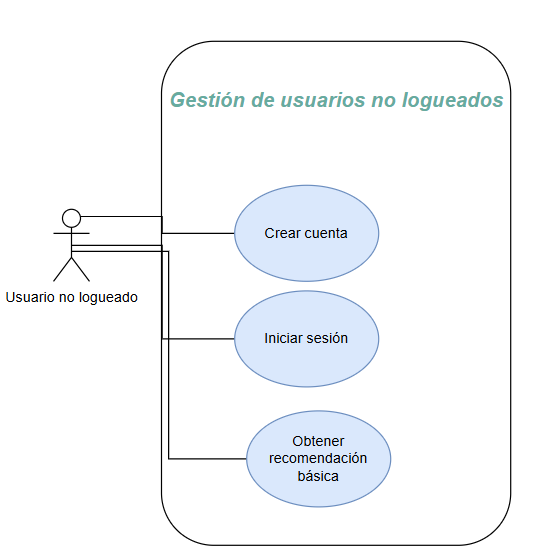
\includegraphics[width=0.75\linewidth]{imagenes/cuU.png}
    \caption{\textbf{Diagrama de casos de uso de usuario no logueado}}
    \label{casos-de-uso-ususario-no-logueado}
\end{figure}
\newpage
\subsection{Casos de uso del usuario logueado}

% Tabla: Caso de uso
\begin{table}[H]
\centering
\begin{tabular}{|c|p{10cm}|}
\hline
\rowcolor{green!40} \textbf{Caso de uso} & CU-04: Modificar información sobre videojuegos. \\ \hline
\rowcolor{blue!10} \textbf{Actores} & ACT-2 (Usuario logueado) \\ \hline
\rowcolor{blue!10} \textbf{Tipo} & Primario \\ \hline
\rowcolor{blue!10} \textbf{Precondición} & - \\ \hline
\rowcolor{blue!10} \textbf{Poscondición} & La información sobre el usuario queda actualizada. \\ \hline
\rowcolor{blue!10} \textbf{Propósito} & Permitir que el usuario modifique su información sobre videojuegos. \\ \hline
\end{tabular}
\caption{Caso de uso de modificar información sobre videojuegos}
\end{table}

% Tabla: Flujo normal de eventos
\begin{table}[H]
\centering
\begin{tabular}{|c|p{5cm}|p{5cm}|}
\hline
\rowcolor{green!40} \textbf{Paso} & \textbf{Actor} & \textbf{Sistema} \\ \hline
\rowcolor{blue!10} 1 & El usuario escribe su modificación en texto y lo envía a los agentes. &  \\ \hline
\rowcolor{blue!10} 2 &  & El sistema recibe la petición y la envía a los agentes, quienes la procesan y toman las medidas oportunas sobre la información de videojuegos del usuario. \\ \hline
\rowcolor{blue!10} 3 &  & El sistema muestra un mensaje indicando que los cambios se han realizado correctamente. \\ \hline
\end{tabular}
\caption{Flujo de eventos del caso de uso CU-04}
\end{table}

% Tabla: Curso alterno de eventos
\begin{table}[H]
\centering
\begin{tabular}{|p{4cm}|p{8cm}|}
\hline
\rowcolor{green!40} \textbf{Curso alterno de eventos} & \textbf{Descripción} \\ \hline
\rowcolor{blue!10} 2a. El texto del usuario no es correcto o está vacío. & El sistema muestra un mensaje de error indicando que el mensaje no es válido. \\ \hline
\end{tabular}
\caption{Curso alternativo del caso de uso CU-04}
\end{table}

% Tabla: Caso de uso
\begin{table}[H]
\centering
\begin{tabular}{|c|p{10cm}|}
\hline
\rowcolor{green!40} \textbf{Caso de uso} & CU-05: Modificar información sobre la cuenta. \\ \hline
\rowcolor{blue!10} \textbf{Actores} & ACT-2 (Usuario logueado) \\ \hline
\rowcolor{blue!10} \textbf{Tipo} & Secundario \\ \hline
\rowcolor{blue!10} \textbf{Precondición} & - \\ \hline
\rowcolor{blue!10} \textbf{Poscondición} & La información sobre la cuenta del usuario queda actualizada. \\ \hline
\rowcolor{blue!10} \textbf{Propósito} & Permitir al usuario modificar su contraseña o nombre de usuario. \\ \hline
\end{tabular}
\caption{Caso de uso de modificar información sobre la cuenta del usuario}
\end{table}

% Tabla: Flujo normal de eventos
\begin{table}[H]
\centering
\begin{tabular}{|c|p{5cm}|p{5cm}|}
\hline
\rowcolor{green!40} \textbf{Paso} & \textbf{Actor} & \textbf{Sistema} \\ \hline
\rowcolor{blue!10} 1 &  & El sistema pide al usuario la contraseña actual. \\ \hline
\rowcolor{blue!10} 2 & El usuario escribe la contraseña actual. & \\ \hline
\rowcolor{blue!10} 3 & El usuario escribe la nueva contraseña y/o el nuevo nombre de usuario. & \\ \hline
\rowcolor{blue!10} 4 &  & El sistema recibe los datos y efectúa el cambio. \\ \hline
\end{tabular}
\caption{Flujo de eventos del caso de uso CU-05}
\end{table}

% Tabla: Curso alterno de eventos
\begin{table}[H]
\centering
\begin{tabular}{|p{4cm}|p{8cm}|}
\hline
\rowcolor{green!40} \textbf{Curso alterno de eventos} & \textbf{Descripción} \\ \hline
\rowcolor{blue!10} 2a. La contraseña no es correcta. & El sistema muestra un mensaje de error indicando que la contraseña es incorrecta y pide que la introduzca nuevamente. \\ \hline
\rowcolor{blue!10} 4a. La nueva contraseña no cumple con los requisitos y/o el nuevo nombre de usuario ya está en uso. & El sistema muestra un mensaje de error indicando que la contraseña no cumple con los requisitos y/o el nuevo nombre de usuario ya está en uso, y pide que se modifiquen los datos. \\ \hline
\end{tabular}
\caption{Curso alternativo del caso de uso CU-05}
\end{table}

% Tabla: Caso de uso
\begin{table}[H]
\centering
\begin{tabular}{|c|p{10cm}|}
\hline
\rowcolor{green!40} \textbf{Caso de uso} & CU-06: Eliminar cuenta. \\ \hline
\rowcolor{blue!10} \textbf{Actores} & ACT-2 (Usuario logueado) \\ \hline
\rowcolor{blue!10} \textbf{Tipo} & Primario \\ \hline
\rowcolor{blue!10} \textbf{Precondición} & - \\ \hline
\rowcolor{blue!10} \textbf{Poscondición} & La cuenta y los datos del usuario han sido eliminados. \\ \hline
\rowcolor{blue!10} \textbf{Propósito} & Eliminar la cuenta del usuario. \\ \hline
\end{tabular}
\caption{Caso de uso de eliminar la cuenta del usuario}
\end{table}

% Tabla: Flujo normal de eventos
\begin{table}[H]
\centering
\begin{tabular}{|c|p{5cm}|p{5cm}|}
\hline
\rowcolor{green!40} \textbf{Paso} & \textbf{Actor} & \textbf{Sistema} \\ \hline
\rowcolor{blue!10} 1 &  & El sistema pide al usuario la contraseña actual. \\ \hline
\rowcolor{blue!10} 2 & El usuario escribe la contraseña actual. & \\ \hline
\rowcolor{blue!10} 3 &  & El sistema pregunta si el usuario está seguro de eliminar su cuenta. \\ \hline
\rowcolor{blue!10} 4 & El usuario confirma. & \\ \hline
\rowcolor{blue!10} 5 &  & El sistema cierra sesión al usuario y borra su cuenta y su información. \\ \hline
\end{tabular}
\caption{Flujo de eventos del caso de uso CU-06}
\end{table}

% Tabla: Curso alterno de eventos
\begin{table}[H]
\centering
\begin{tabular}{|p{4cm}|p{8cm}|}
\hline
\rowcolor{green!40} \textbf{Curso alterno de eventos} & \textbf{Descripción} \\ \hline
\rowcolor{blue!10} 2a. La contraseña no es correcta. & El sistema muestra un mensaje de error indicando que la contraseña es incorrecta y la pide de nuevo al usuario. \\ \hline
\rowcolor{blue!10} 3a. El usuario no está seguro de eliminar la cuenta. & El sistema regresa al usuario a la sección anterior. \\ \hline
\end{tabular}
\caption{Curso alternativo del caso de uso CU-06}
\end{table}

% Tabla: Caso de uso
\begin{table}[H]
\centering
\begin{tabular}{|c|p{10cm}|}
\hline
\rowcolor{green!40} \textbf{Caso de uso} & CU-07: Obtener datos con API externa. \\ \hline
\rowcolor{blue!10} \textbf{Actores} & ACT-2 (Usuario logueado) \\ \hline
\rowcolor{blue!10} \textbf{Tipo} & Primario \\ \hline
\rowcolor{blue!10} \textbf{Precondición} & Tener una cuenta en la plataforma externa. \\ \hline
\rowcolor{blue!10} \textbf{Poscondición} & La plataforma obtiene y guarda los datos de videojuegos de la plataforma externa. \\ \hline
\rowcolor{blue!10} \textbf{Propósito} & Obtener información de plataformas externas. \\ \hline
\end{tabular}
\caption{Caso de uso de obtener datos con API externa}
\end{table}

% Tabla: Flujo normal de eventos
\begin{table}[H]
\centering
\begin{tabular}{|c|p{5cm}|p{5cm}|}
\hline
\rowcolor{green!40} \textbf{Paso} & \textbf{Actor} & \textbf{Sistema} \\ \hline
\rowcolor{blue!10} 1 & El usuario pide conectarse a la API. &  \\ \hline
\rowcolor{blue!10} 2 &  & El sistema llama a la API. \\ \hline
\rowcolor{blue!10} 3 &  & \#Include api. \\ \hline
\rowcolor{blue!10} 4 &  & El sistema recibe el resultado de la API y almacena la información obtenida. \\ \hline
\end{tabular}
\caption{Flujo de eventos del caso de uso CU-07}
\end{table}

% Tabla: Caso de uso
\begin{table}[H]
\centering
\begin{tabular}{|c|p{10cm}|}
\hline
\rowcolor{green!40} \textbf{Caso de uso} & CU-08: Obtener recomendaciones personalizadas. \\ \hline
\rowcolor{blue!10} \textbf{Actores} & ACT-2 (Usuario logueado) \\ \hline
\rowcolor{blue!10} \textbf{Tipo} & Primario \\ \hline
\rowcolor{blue!10} \textbf{Precondición} & - \\ \hline
\rowcolor{blue!10} \textbf{Poscondición} & El usuario obtiene recomendaciones según su información y lo preguntado. \\ \hline
\rowcolor{blue!10} \textbf{Propósito} & Obtener recomendaciones personalizadas. \\ \hline
\end{tabular}
\caption{Caso de uso de obtener recomendaciones personalizadas}
\end{table}

% Tabla: Flujo normal de eventos
\begin{table}[H]
\centering
\begin{tabular}{|c|p{5cm}|p{5cm}|}
\hline
\rowcolor{green!40} \textbf{Paso} & \textbf{Actor} & \textbf{Sistema} \\ \hline
\rowcolor{blue!10} 1 & El usuario escribe su petición. &  \\ \hline
\rowcolor{blue!10} 2 &  & El sistema pasa la petición a los LLMs junto a la información del usuario, y estos la procesan, almacenan y crean una respuesta. \\ \hline
\rowcolor{blue!10} 3 &  & El sistema devuelve la respuesta al usuario. \\ \hline
\end{tabular}
\caption{Flujo de eventos del caso de uso CU-08}
\end{table}

% Tabla: Curso alterno de eventos
\begin{table}[H]
\centering
\begin{tabular}{|p{4cm}|p{8cm}|}
\hline
\rowcolor{green!40} \textbf{Curso alterno de eventos} & \textbf{Descripción} \\ \hline
\rowcolor{blue!10} 2a. & La petición es invalida. El sistema pide  al usuario que la introduzca de nuevo.\\ \hline
\end{tabular}
\caption{Curso alternativo del caso de uso CU-08}
\end{table}
\newpage
\subsection{Casos de usos de administrador}

Similar ausuario logueado, pero con acceso a información de debugueo, opciones especiales...

% Tabla: Caso de uso
\begin{table}[H]
\centering
\begin{tabular}{|c|p{10cm}|}
\hline
\rowcolor{green!40} \textbf{Caso de uso} & CU-09: Opciones avanzadas y obtener métricas. \\ \hline
\rowcolor{blue!10} \textbf{Actores} & ACT-3 (Administrador) \\ \hline
\rowcolor{blue!10} \textbf{Tipo} & Primario \\ \hline
\rowcolor{blue!10} \textbf{Precondición} & - \\ \hline
\rowcolor{blue!10} \textbf{Poscondición} & El administrador obtiene métricas. \\ \hline
\rowcolor{blue!10} \textbf{Propósito} & Obtener métricas y ejecutar opciones avanzadas. \\ \hline
\rowcolor{blue!10} \textbf{Extiende} & CU-04 $\rightarrow$ CU-09.\\ \hline
\end{tabular}
\caption{Caso de uso de Opciones avanzadas y obtener métricas}
\end{table}

% Tabla: Flujo normal de eventos
\begin{table}[H]
\centering
\begin{tabular}{|c|p{5cm}|p{5cm}|}
\hline
\rowcolor{green!40} \textbf{Paso} & \textbf{Actor} & \textbf{Sistema} \\ \hline
\rowcolor{blue!10} 1 & El administrador pide ejecutar un método, con posibles opciones avanzadas. &  \\ \hline
\rowcolor{blue!10} 2 &  & El sistema ejecuta ese método con las opciones avanzadas especificadas, además de ofrecer métricas. \\ \hline
\end{tabular}
\caption{Flujo de eventos del caso de uso CU-09}
\end{table}

\clearpage 

\begin{figure}[H]
    \centering
    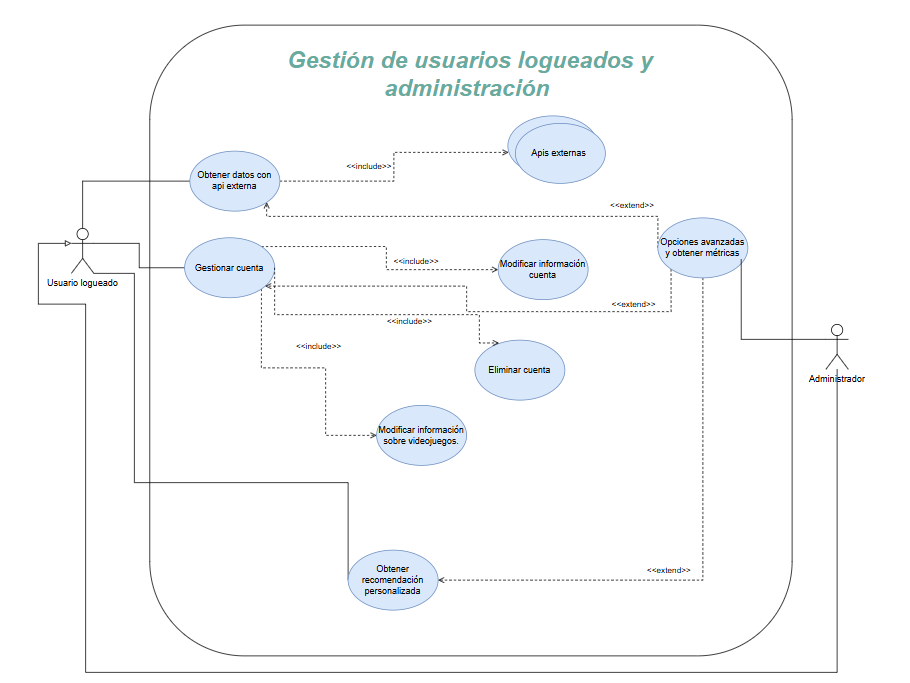
\includegraphics[width=1.3\linewidth]{imagenes/cuULYA.png}
    \caption{\textbf{Diagrama de casos de uso de usuario logueado y administrador}}
    \label{casos-de-uso-usuario-logueado}
\end{figure}








